% The central motivation for the computational part: responsibility precedes reliance on assistance.
\begin{abwfigureframe}{Why learn Python now?}{\ABWInsertedPageNumber}
  \node[anchor=north west,inner sep=0pt,outer sep=0pt] at (40.625,-139)
    {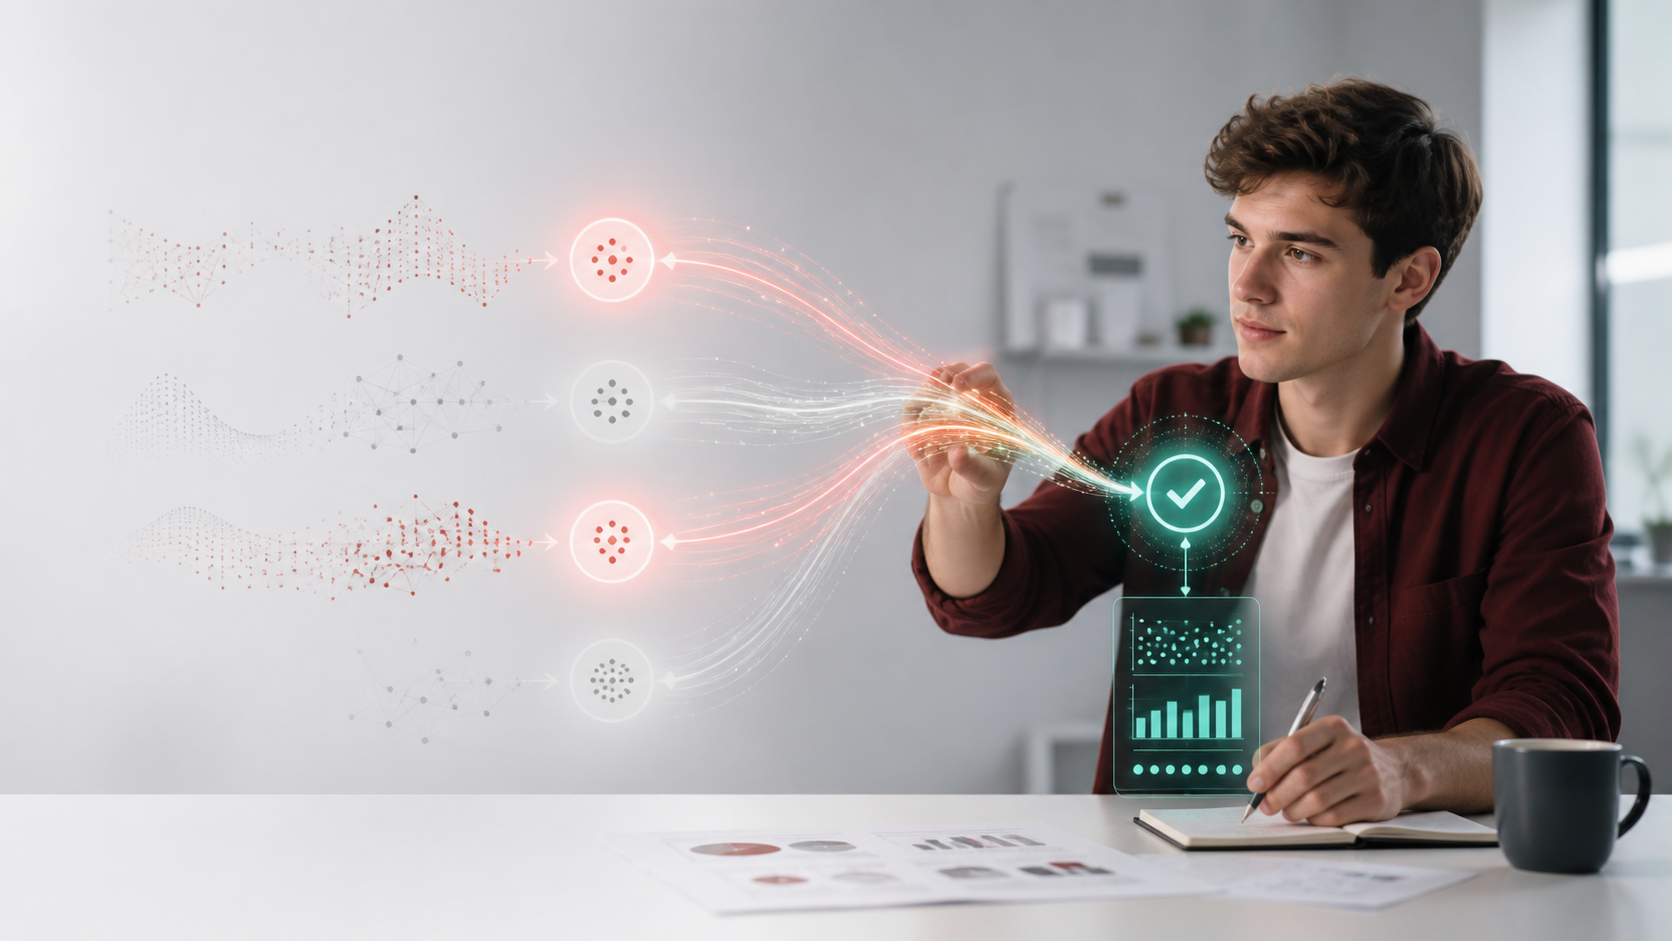
\includegraphics[width=878.75bp,height=322bp]{assets/ai/human-directs-ai.png}};
  \fill[white,draw=none] (56,-157) rectangle (444,-442);
  \node[anchor=north west,inner sep=0pt,text width=346bp] at (78,-177)
    {{\TimesNR\fontsize{24}{29}\selectfont\raggedright
      AI may draft code, suggest models, and summarize results.\par\vspace{22bp}
      \color{ABWRed}\bfseries You need enough fluency to:\par\vspace{10bp}
      \color{black}\normalfont
      \ABWPersonBullet{Specify the problem and assumptions.}
      \ABWPersonBullet{Read and test what the code does.}
      \ABWPersonBullet{Correct mistakes and own the decision.}
    }};
  \node[anchor=east,inner sep=0pt] at (903,-475)
    {{\TimesNR\fontsize{9}{11}\selectfont\color{ABWGray}Project-generated conceptual artwork, August 2026}};
\end{abwfigureframe}
